\chapter{Design}

\begin{flushleft}
The following chapter details the design of the data gathering Android application. It will also outline the sever side implementation to compute, store and provide information. Afterwards follows a short description of some additional tools, needed for the data analysis.\\
First, it will start with a brief description of the two components and will follow with my design decisions and my reasons for the choices. 
\end{flushleft}

\section{Approach}
This approach has been created to be a possible base for a system that helps to improve the working behavior and environment of developers. 
In this dissertation we created a toolset that allows to gather data from the mobile phone of the participants, analyze it and correlate it with the code quality of their work. The technical design for this approach is created for the experimental data gathering of a limited amount of participants. The described system is not capable to handle high traffic and to analyze the data entries of great amount of users. 

\section{Functionality Overview}
The name of the application was chosen to be "Dather", which is a a combination of "Data" and "Gather".
The purpose of the application is to gather information from a mobile device of a participant while he/she is working on a programming task. Afterwards the application sends the collected data to a server for further processing and analysis. The participant also simultaneously submits the written code which code quality will be detected and then correlated with the processed mobile device information. 

\section{Mobile Application Design}
% Define bar chart colors
\definecolor{others}{HTML}{e78d1c}
\definecolor{android}{HTML}{a4c639}
\definecolor{ios}{HTML}{1c90e7}

\begin{figure}
	\centering
	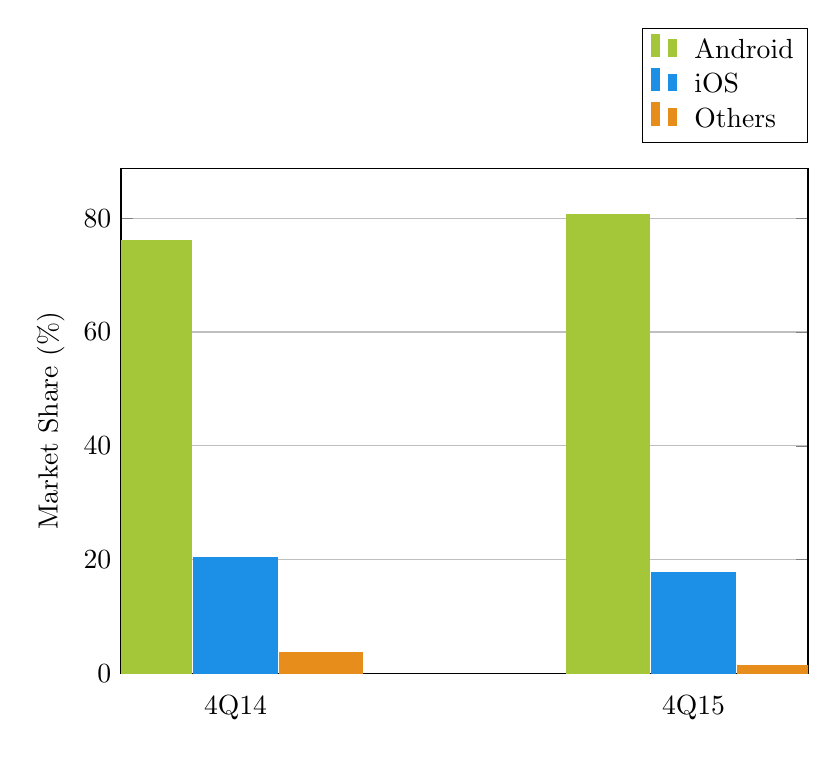
\begin{tikzpicture}
        \begin{axis}[
            width  = 0.85*\textwidth,
        	height = 8cm,
        	major x tick style = transparent,
        	ybar=2*\pgflinewidth,
        	bar width=30pt,
        	ymajorgrids = true,
        	ylabel = {Market Share (\%)},
        	symbolic x coords={4Q14, 4Q15},
       	 	xtick = data,
        	scaled y ticks = false,
        	enlarge x limits=0.25,
        	ymin=0,
        	legend cell align=left,
        	legend style={
                at={(1,1.05)},
                anchor=south east,
                column sep=1ex
        	}
      	]
     	\addplot[style={android,fill=android,mark=none}]
            coordinates {(4Q14, 76.0) (4Q15, 80.7)};

        \addplot[style={ios,fill=ios,mark=none}]
             coordinates {(4Q14, 20.4) (4Q15, 17.7)};

        \addplot[style={others,fill=others,mark=none}]
             coordinates {(4Q14, 3.7) (4Q15, 1.5)};

        \legend{Android, iOS, Others}

        \end{axis}
 	\end{tikzpicture}
 	\caption{Smartphone OS Marketshare}\label{result}
 	\vspace{10 mm}
\end{figure}

\begin{flushleft}
In quarter 4 of 2015 Android had a market share of 80.7\% in smart-phone sales by operating system (see Figure \ref{result}). The trend also shows that the number increased from the last year \cite{gartnerMobileOSMarketshare}. Therefore I decided to realize the mobile application implementation for Android in order to be able to work with more users who have access to that application.\\
An alternative to the native implementation (e.g. iOS or Android) could have been a hybrid application. A hybrid apps is based on web-technology and using the addvantage of resposive web design to be able to work with every aspect ratio and resolution on an mobile device. One way doing that would be by using a framework such as PhoneGap, wich internally creates a native webview applicationand just loads the hybrid JavaScript, HTML, CSS in it. Another software for cerating a hybrid solution is Titanum accelerator which itself is using native UI components. Both frameworks have the advantage is the simple development and the OS independence. The problem with hybrid apps are the performance and limited accessiblity to hardware components including some sensors \cite{holzinger2012making}.  
\bigbreak
The Android application make use of its build-in sensors and information provided by the Android operating system \ref{sensors}. Different than iOS, Android is an OS that can be installed of different devices from various manufactorers and with different hardware components \cite{goadrich2011smart}. Thus, the buit-in sensors which are clustered in motion sensors, environmental sensors and position sensors \cite{androidDevelopers} can differ between the diverse devices. Components that are required for standard functionality such as making phone calls are more common than other sensors. For example, the microphone for recording the users voice or the light sensor, which is used to detect whether the user has the phone at his ear can be found in almost every mobile android device. 
Furthermore, the different mobile device manufacturers customize the open source android operating system for their devices and their purposes. This nature can lead to different settings or behavior for the hardware and also software components.\\
This device diversity and the variety of different screen sizes and aspect ratios make it more difficult to support a range of android devices and make sit impossible to test all devices that are running a specific operating system. Apple at the other hand uses the same aspect ration up from the iPhone5 and supports the hardware components in a similar way in iOS. 
\end{flushleft}

\begin{figure}
\centering
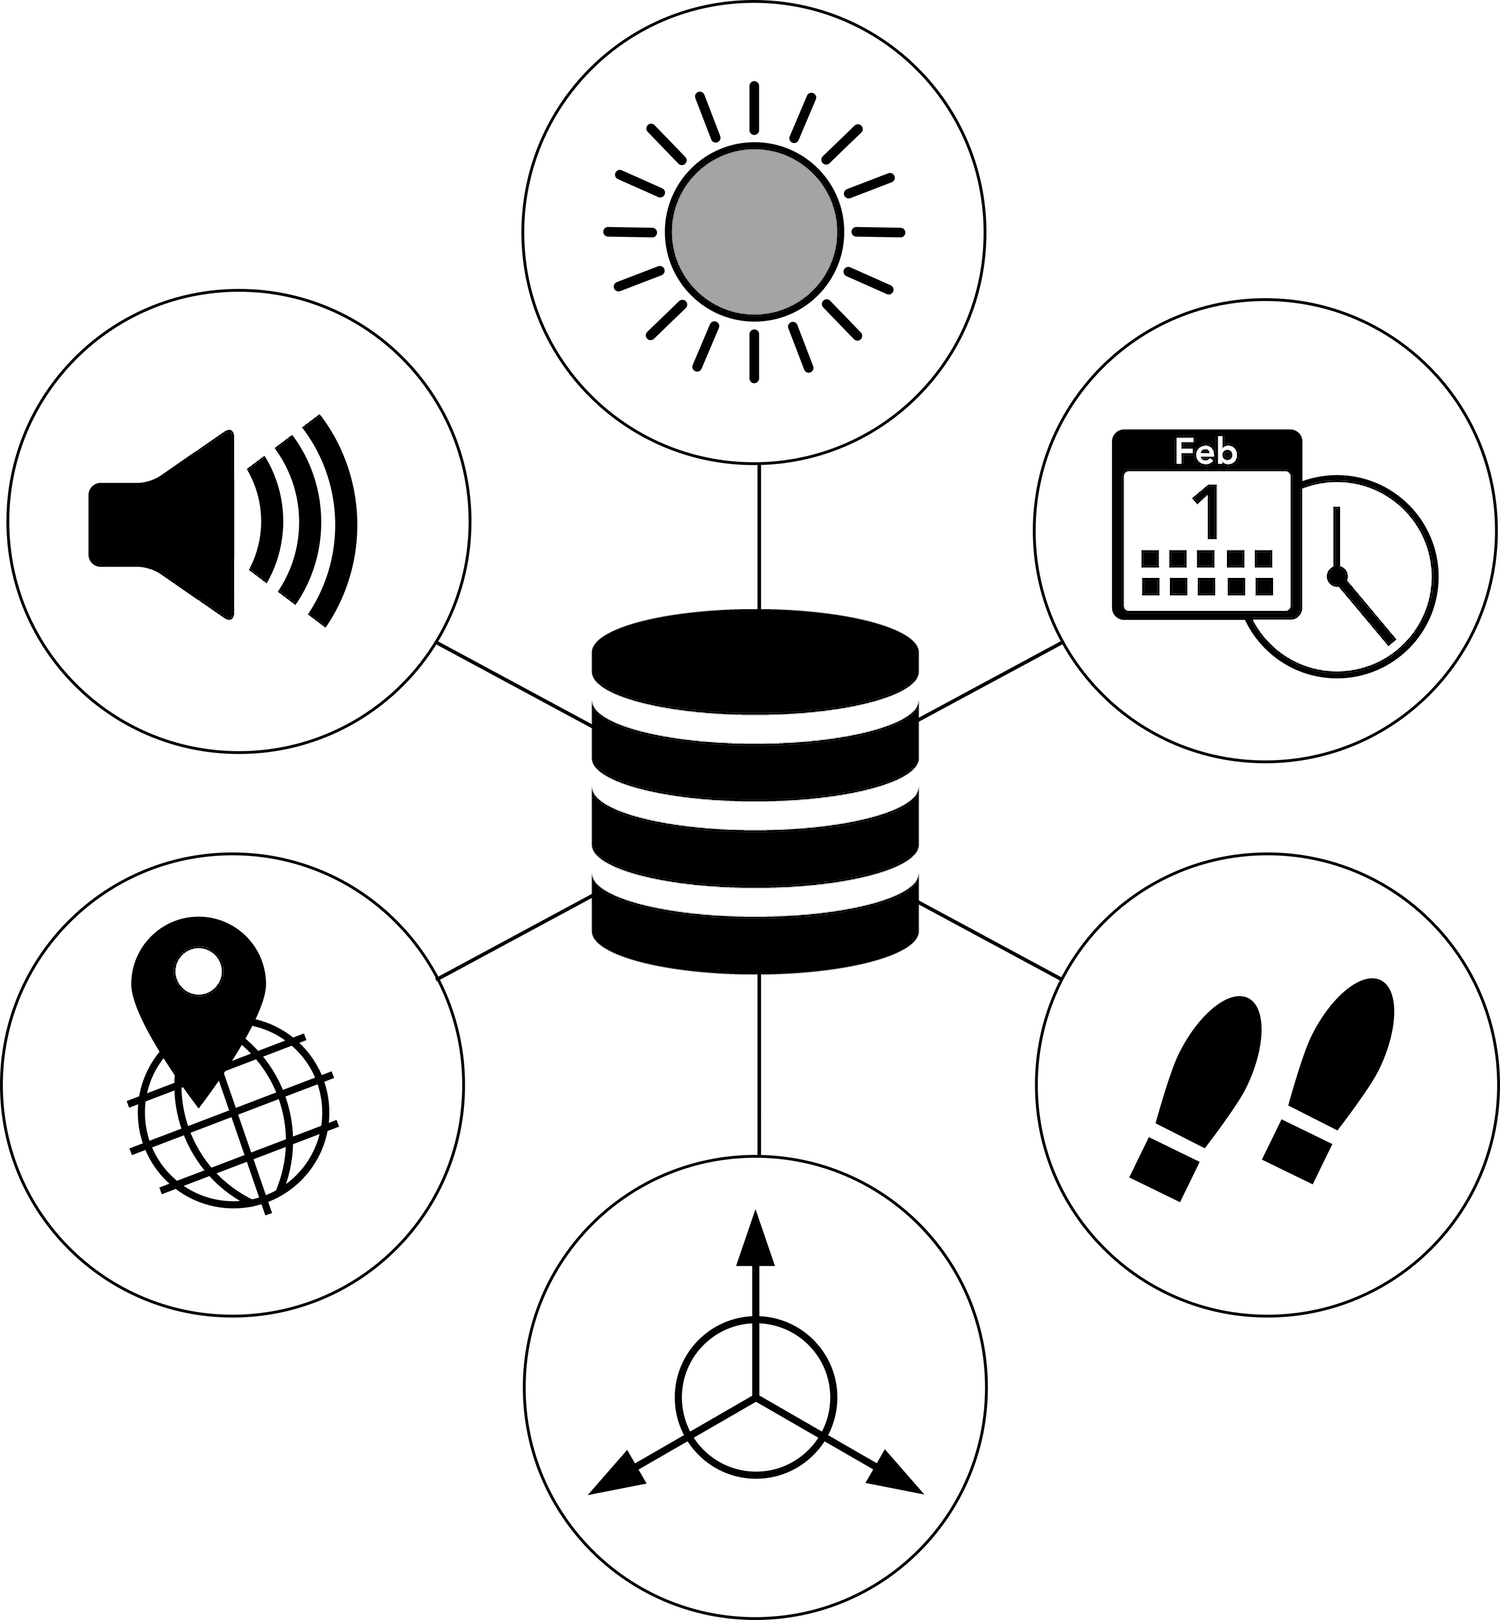
\includegraphics[width=8 cm]{sensors}
\caption{gather data: light, timestamp, steps, accelerometer, location, volume}\label{sensors}
\vspace{5 mm}
\end{figure}

\subsection{Requirements}
The application is primarily created for the research project and therefore not for the everyday use. The participants should not waste much time in finding out how the app works. The goal was to create a simple and intuitive interface and a leading flow trough the functionality. The apps purpose is to gather the data of the participant during coding. That includes the usage of the mobile device during work. Thus, the gathering app must be able to run in the background, so the participant can use the app as he/she would normally do (e.g. Listing to music, texting etc.)

\subsection{App Architecture}
The Android app is built based on the Model View Controller design principles. This design principle defines the interfaces between the three different parts, the Model, the View and the Controller and states the tasks and responsibilities of each part.\\
The Model is the data source and in this app represented by the SQLite Database and can only communication happens to the Controller. 
The Controllers are called Activities in the Android Framework and is responsible for managing the Views, which are defined in XML files and then modified by the responsible Controller. 
To keep the code base clean and to avoid bugs, the communication is separated by the controller. The Model doesn't directly communicate with the View and can't update it. It the case of changes, the Model informs the Controller, which decides whether or not to update the view etc. 

\subsection{User Interface}

\begin{figure}
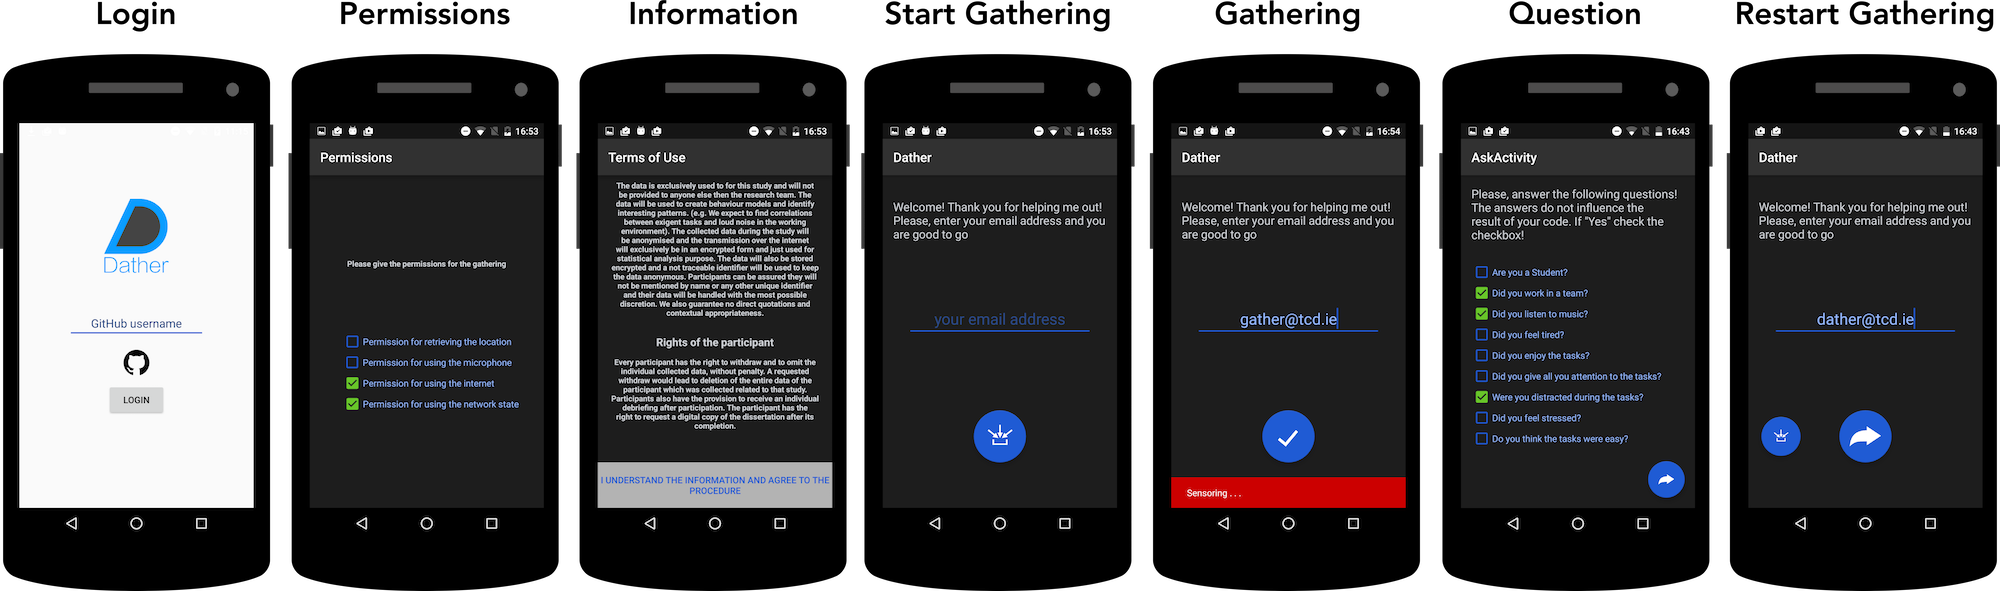
\includegraphics[width=\textwidth]{AndroidUI}
\caption{Android Views}\label{aviews}
\vspace{10 mm}
\end{figure}

The Application has two main user Interfaces, the gathering view and the question view.\\
The gathering view is the control interface for starting, stopping and transmitting the data gathering. The appearance of the user interface changes related the current state and the logical functionality. 
This view also displays the username and a short informing text.
\bigbreak
After successfully sending the gathered data to the server the application displays the question view. Here, the user sees a number of questions and check-boxes to answer the binary yes and no questions. 
This interface also provides a send button to submit the answered questions to the Server.
\bigbreak
In Figure \ref{aviews} you can see the flow of the views in the applications.
It shows screenshots of the flow within the app from left to right. Starting at the login view, where the participant enters his/her Github username. 
The next view asks for the permissions followed by the view that informs about the sensible data handling. 
In the middle you can see the gathering view, where the user controls the process. The right screenshot shows the gathering process in action. The next view contains the questions to the user. The last view shows the gathering view with a changed functionality. Here the user can gather data again after completing the first gathering process. 

\subsection{Data Storage}
For storing the gathered data entries, the app uses a SQLite datebase. SQLite uses SQL syntax which and is embedded in Android and well documented by Google. \cite{vogel2010android}. It is a very light weight database and provides an abstracted and easy way to store the values in an object oriented environment. SQLite is storing the data unencrypted by default. In order to make sure the stored data is save and can't be read, the data is been encrypted as soon it's been gathered.\\
The database has a capacity of 1024 MB which is equal to 1,000,000 KiB and can store 2,380,952 entries of an average of 0.42 KiB (this value is calculated based on the used storage of 1,000 entries). Assuming that the maximum gathering get 30 entries per minute, the database can store 7,9365.07 minutes or 1,322.75 hours of the gathered data.\\
\\bigbreak
Additional to the SQLite database, Android provides a way to store single entries such as the field with the email address of the user. The so called "shared preferences" are storing key-value-pairs persistently on the phone and can be accessed from everywhere in the application.


\subsection{API}
The gathered data and afterwards the answered questions will asynchronously send to the Server and written into the database. When the response will be received, the view shows a visual confirmation and moves on to the next step or in case of the questions back to the gathering interface. 
\bigbreak
The communication to the Server uses HTTP connection over a stateless REST-full service. The REST-Service is a centralized way to allow making entries to the database and use the computing power of the server. PHP is the programming language used server-side and is establishing the connection to the MYSQL database.\\
As this application just requires to send information to the server but not receive information, the data gets converted to JSON format and send to the server via a POST request. The server response with a success or fail and provides some additional information in case entries were added to the database. 

\subsection{User Information}
For accessing the information from the mobile device, Android requires the user to granting the permissions for specific functionality such as using using the internet connection of the phone or access information like the telephone book entries.\\
The permissions were given when the the user by simply downloading the app from the PlayStore all in one place. However, since Android 6, the developer now is forced to ask for the permissions within the application itself  \cite{androidpermissions}.\\
Thus, the users with Android 6 or higher are provided by a additional interface which is specifically asking for permissions for Internet Access, access internet state information, using the device microphone and getting the location of the device. 
\bigbreak
Independent from the Android version the user needs to read and accept the terms of use at the first start of the application. The displayed text informs the user about the rights and what is happening with the data and information the user provides through this app usage.
\bigbreak
Within the app the user is asked to enter his/her email address. The email address then is being hashed with the SHA256 algorithm to ensure the data will be anonymous and can't connected to the user.   
\bigbreak
Also the gathered data are stored encrypted in the SQLite database on the mobile device and just decrypted on a local computer after the researchers downloaded the encrypted entries from the SQL database on the server. That ensure that the files are not accessible in readable format at any time. 

\section{Server Design}
The server is hosted by 1\&1 Internet SE as a completely pre-configured server backend PHP version 5.6 and the MYSQL-server phpMyAdmin in version 4.1.14.8. The also pre-configured server file system can be accessed using SSH or via FTP.

\subsection{requirements}
The Website is required to provide all the information a participant could need to do the experiment. The Interface should be clean and the participant should be also able to download the android application from the same website as he/she gets the information about the experiment. 
The backend will only be used by the researchers and therefore the user interface doesn't matter as much as for the participants. The functionality and the customization are the most important features. 

\subsection{Server Frontend Design}
The information for the participants of the study can access information web pages and access the downloadable Android application.\\
The frontend is implemented in HTML5 and CSS3 and simply uploaded to the server. As everything is public available and accessible there was no need or using a framework or any further security implementation. 

\subsection{Server Backend Design}
The backend is implemented in PHP with the MYSQL-server phpMyAdmin database.\\ 
No external frameworks have been used to implement the basic REST-full service and the establishing of the database connection and the SQL queries.

\section{Tools}
The following tools are were used during the experiment primarily for the decryption of data to automate some processes.

\subsection{requirements}
The tools are also just for the usage of the researchers and the requirements therefor also the functionality, the security that no information are getting lost.

\subsection{Decrypting Tool}
The encryption tool an executable program written in Java for locally encrypting the downloaded gathered data.\\
Its interface contains of an input field for the path of the downloaded data in JSON-format, a button for first reading and afterwards decrypting and a output text that shows the current state of the application. The tool writes the decrypted input values in a separate text file in the same directory of the input file with the same name but with the file extension .txt instead of .json. 

\subsection{Data Structuring Tools}
For working with the resulting data from the experiment, a tool-set was created to take over specific tasks. All the tools for this purpose are implemented in Python because it provides a very handy way to work with external files. 
The first tool allows to extract only the entries from a specific participant by providing the his/her Github username.\\
Another tool extracts the single values per entry with its timestamp and the last tool averages the results per minute and converts the data into a form that can directly be used in latex to draw plots.

\section{Future Work}
Based on the experience and the learning from this approach, we want to enable further work on system that could be used to gather data from the developers and provide them a real-time feedback on their code and ways to improve their performance.
A external hardware device with a collection of sensors, placed on the developers desk could gather additional to the mobile device. 
The combined information could be constantly analyzed on a server and compared to the data of other developers. Automatic learning algorithms could compare the gathered data and the code of the developers to find more specific trends and influencing factors in the performance. 
Furthermore, notifications from the server to the device of the developer could provide feedback and tips for improvement by mentioning the influences. 

\section{Summary}
This chapter is about the design decisions of the different software parts that are needed for the experiments. First, the functionality of each part are being described, followed by the part about the Android application. Android was the mobile OS of choice because it has the highest market share of all mobile operating systems. The app needs to be simple and easy to use for single usage which is seen in the UI and the UX specification. 
The app was programmed in Java using the MVC design pattern while using an SQLite database for the permanent data storage. The app-server communication is been realized using a REST-API and in order to do nothing against the users will, the user needs to grand permissions and accept term to be able to use the app. \\
The Server backend is implemented in PHP with an MySQL database while the frontend is implemented in HTML5 and CSS while the decryption tool was created in java and the rest tools in python. 